\documentclass[9pt]{extarticle}   	% use "amsart" instead of "article" for AMSLaTeX format
\usepackage{geometry}
 \geometry{
 a4paper,
 total={170mm,257mm},
 top=20mm,
 left=20mm,
 top=20mm,
 bottom=20mm,
 }%\geometry{landscape}                		% Activate for rotated page geometry
%\usepackage[parfill]{parskip}    		% Activate to begin paragraphs with an empty line rather than an indent
\usepackage{graphicx}				% Use pdf, png, jpg, or eps§ with pdflatex; use eps in DVI mode
								% TeX will automatically convert eps --> pdf in pdflatex		
\usepackage{amssymb}
\usepackage{natbib}
%\setlength{\textfloatsep}{-10cm}

\usepackage{hyperref}

\def\multic#1#2{\multicolumn{#1}{c}{#2}}
\def\dagmark{\multic{1}{$\dag$\qquad}}


\def\aj{{AJ}}                  % Astronomical Journal
\def\araa{{ARA\&A}}            % Annual Review of Astron and Astrophys
\def\apj{{ApJ}}                        % Astrophysical Journal
\def\apjl{{ApJ}}               % Astrophysical Journal, Letters
\def\apjs{{ApJS}}              % Astrophysical Journal, Supplement
\def\ao{{Appl.Optics}}         % Applied Optics
\def\apss{{Ap\&SS}}            % Astrophysics and Space Science
\def\aap{{A\&A}}               % Astronomy and Astrophysics
\def\aapr{{A\&A~Rev.}}         % Astronomy and Astrophysics Reviews
\def\aaps{{A\&AS}}             % Astronomy and Astrophysics, Supplement
\def\azh{{AZh}}                        % Astronomicheskii Zhurnal
\def\baas{{BAAS}}              % Bulletin of the AAS
\def\jrasc{{JRASC}}            % Journal of the RAS of Canada
\def\memras{{MmRAS}}           % Memoirs of the RAS
\def\mnras{{MNRAS}}            % Monthly Notices of the RAS
\def\pra{{Phys. Rev. A}}         % Physical Review A: General Physics
\def\prb{{Phys. Rev. B}}         % Physical Review B: Solid State
\def\prc{{Phys. Rev. C}}         % Physical Review C
\def\prd{{Phys. Rev. D}}         % Physical Review D
\def\prl{{Phys. Rev. Lett}}      % Physical Review Letter
\def\pasp{{PASP}}              % Publications of the ASP
\def\pasj{{PASJ}}              % Publications of the ASJ
\def\qjras{{QJRAS}}            % Quarterly Journal of the RAS
\def\rmxaa{{RMxAA}}		%Revista Mexicana de Astronomia y Astrofisica
\def\skytel{{S\&T}}            % Sky and Telescope
\def\solphys{{Solar~Phys.}}    % Solar Physics
\def\sovast{{Soviet~Ast.}}     % Soviet Astronomy
\def\ssr{{Space~Sci.Rev.}}     % Space Science Reviews
\def\zap{{ZAp}}                        % Zeitschrift fuer Astrophysik
\def\nat{{Nature}}             % Nature



\title{Spectral Energy Distribution Reference Tables and Plots}
\author{\textbf{R. E. Ainsworth}, A. M. M. Scaife, D. A. Green, C. P. Coughlan and T. P. Ray, \\ ''GMRT detections of low mass young stars at 323 and 608 MHz'', \\ \textit{Monthly Notices of the Royal Astronomical Society}, 459, 1248--1258, 2016}
\date{}							% Activate to display a given date or no date

\begin{document}
\maketitle


%I conducted an extensive literature search for unresolved, integrated flux densities to include in the spectral energy distribution for each source. It should be noted that \citet{1995A&AS..109..177W} was a useful reference. High resolution data that were highly discrepant due to flux loss or data with high uncertainties \citep[e.g. $450\,\mu$m data from][]{2008ApJS..175..277D} were not included. Spectral energy distributions are shown with the maximum likelihood models from \ref{tab:AMIsrcalpha2} overlaid. The list of archival data used in the spectral energy distributions can be found below. Where uncertainties were not provided, an error of $10$\% was used in the model fittings and this is indicated by a $^{\dag}$. Only data $\nu<3$\,THz ($\lambda>100\,\mu$m) were included in the fit, but \textit{IRAS} data $\nu>3$\,THz are included in the plots for illustration.

%The Markov Chain Monte Carlo based Maximum Likelihood algorithm \textsc{METRO} \citep{hob04} was used to fit a combined radio power-law, with spectral index $\alpha'$, and blackbody model to the larger dataset for each source. This fit utilised data at wavelengths longer than $100\,\mu$m and had the form: 
%\begin{equation}
%S_{\rm total} = S_{1} + S_{2} = K_{1}\left(\frac{\nu}{\nu_{1}}\right)^{\alpha'} + K_{2}\frac{\nu^{\beta}B_{\nu}(T_{\rm{d}})}{\nu_{2}^{\beta}B_{\nu_{2}}(T_{\rm{d}})},
%\end{equation}
%where $\beta$ is the dust opacity index, $B_{\nu}$ is the Planck function for a dust temperature $T_{\rm{d}}$, $K_{1}$ is the normalised flux density at $\nu_{1}=16$\,GHz and $K_{2}$ is the normalised flux density at $\nu_{2}=300$\,GHz. It can be seen that when $\nu=\nu_{1}$, $S_{1}$ equals $K_{1}$, the normalised flux density at $16$\,GHz and when $\nu=\nu_{2}$, $S_{2}$ equals $K_{2}$, the normalised flux density at $300$\,GHz, and we define these parameters as $S_{16}^{\rm norm}$ and $S_{300}^{\rm norm}$ respectively. Uniform and separable priors were used for all parameters, with ranges
%\begin{equation}
%\Pi=\Pi_{\alpha}(-2,2)\Pi_{\beta}(0,3)\Pi_{T_{\rm d}}(5,45).
%\end{equation}


An extensive literature search was conducted for integrated flux densities (on scales comparable with the GMRT) to include in the spectral energy distributions following \citet{2012MNRAS.423.1089A}. Where uncertainties were not provided, an error of 10\,per~cent was used in the model fittings and this is indicated by a $^{\dag}$. The reference list for the flux densities used in the L1551~IRS~5 spectral energy distribution (for $\nu<1$\,THz and in addition to the data presented in this work), can be found in the online supplementary material of \citet{2012MNRAS.423.1089A} or \url{https://github.com/rainsworth/Spectral-Energy-Distributions/tree/master/2012MNRAS.423.1089A}.

The Markov Chain Monte Carlo based Maximum Likelihood algorithm \textsc{metro} \citep{hob04} was used to fit a combined double power-law to the larger dataset of each source to model the two apparent emission components: free--free emission from the partially ionised outflow (with low frequency spectral index $\alpha$) and thermal dust emission from the circumstellar disc/envelope (with high frequency spectral index $\alpha'$) using a joint likelihood. It is important to disentangle these two emission mechanisms simultaneously as it has been shown that considering free--free and thermal dust components separately can give vastly different values for the spectral slope and normalisation of each component \citep[e.g.][]{2012MNRAS.420.3334S}. This can have implications when determining physical parameters from the free--free spectra (such as gas mass and electron density) and the thermal dust spectra (such as disc mass and grain size).

In the Rayleigh--Jeans region ($h\nu \ll k_{\rm B}T_{\rm d}$, or $\nu\ll1$\,THz for a characteristic dust temperature $T_{\rm d}=50$\,K), the thermal emission from dust grains in the circumstellar environment can be well approximated by a power-law with $S_\nu \propto \nu^{\alpha'}$ \citep[e.g.][]{2013MNRAS.435.1139S}. The spectral index $\alpha'$ of flux density measurements is related to the dust opacity index $\beta$ as $\beta \simeq (1+\Delta)\times(\alpha'-2)$, where $\Delta$ is the ratio of optically thick to optically thin emission \citep{1990AJ.....99..924B}. At long wavelengths $\Delta \rightarrow 0$ as the emission is entirely optically thin, so $\beta\approx\alpha'-2$. This allows the largest grain sizes to be determined directly from a measure of this spectral index. 

The fitted model is of the form,
\begin{equation}
\left( \frac{S_\nu}{\rm mJy} \right) = K_{323\,\rm{MHz}} \left( \frac{\nu}{\rm 323\,MHz} \right)^\alpha + K_{100\,\rm{GHz}} \left( \frac{\nu}{\rm 100\,GHz} \right)^{\alpha'},
\end{equation}
where the constants $K_{323\,\rm{MHz}}$ and $K_{100\,\rm{GHz}}$ normalise the two power-law components at 323\,MHz and 100\,GHz ($\lambda=90$\,cm and 3\,mm, respectively). Consequently, $K_{323\,\rm{MHz}}$ represents the normalised flux density at 323\,MHz (expected to be dominated by free--free emission) and $K_{100\,\rm{GHz}}$ represents the normalised flux density at 100\,GHz (expected to be dominated by thermal dust emission).  

We fit all the available flux densities for each target source using uniform separable priors such that,
\begin{equation}
\Pi = \pi_{K_{323\,\rm{MHz}}}(0, 10\,{\rm mJy})~\pi_{\alpha}(-2, 2)~\pi_{K_{100\,\rm{GHz}}}(0, 1\,{\rm Jy})~\pi_{\alpha'}(0, 4). \nonumber
\end{equation}
The prior range for $\alpha$ was selected to allow a variety of possible radio emission mechanisms such as synchrotron ($\alpha\lesssim-0.7$), optically thin free--free ($\alpha\approx-0.1$) and optically thick free--free ($\alpha\approx2$). The prior range for $\alpha'$ was chosen to allow a range of values up to $\beta=2$ expected for protostellar envelopes with small, warm dust grain populations \citep[e.g.][]{2013MNRAS.435.1139S}. The prior ranges for $K_{323\,\rm{MHz}}$ and $K_{100\,\rm{GHz}}$ were chosen based on the flux densities of these objects around 323\,MHz and 100\,GHz. 

\vspace{10mm}
\begin{table}[h!]
\centering
\caption{SED modelling results. Column [1] contains the target source name; [2] the derived normalisation of the low frequency power-law at 323\,MHz; [3] the derived low frequency spectral index $\alpha$; [4] the derived normalisation of the high frequency power-law at 100\,GHz; and [5] the derived opacity index $\beta$ which is related to the high frequency spectral index $\alpha'$ as $\beta\approx\alpha'-2$.}
\label{tab:SEDresults}
\begin{tabular}{lcccc} 
\hline
Source & $K_{323\,\rm{MHz}}$ & $\alpha$ & $K_{100\,\rm{GHz}}$ & $\beta$  \\
	& (mJy) & & (mJy) & \\ 
\hline
L1551~IRS~5 	& $1.61\pm0.10$ & $0.23\pm0.02$ & $120.58\pm3.63$ & $1.31\pm0.05$  \\
T~Tau 		& $3.43\pm0.08$ & $0.17\pm0.01$ & $28.16\pm1.15$ & $0.56\pm0.03$  \\
DG~Tau 		& $0.55\pm0.05$ & $0.20\pm0.03$ & $34.54\pm1.08$ & $0.55\pm0.03$  \\
\hline
\end{tabular}
\end{table}


\clearpage

\begin{figure}[h!]
\begin{center}
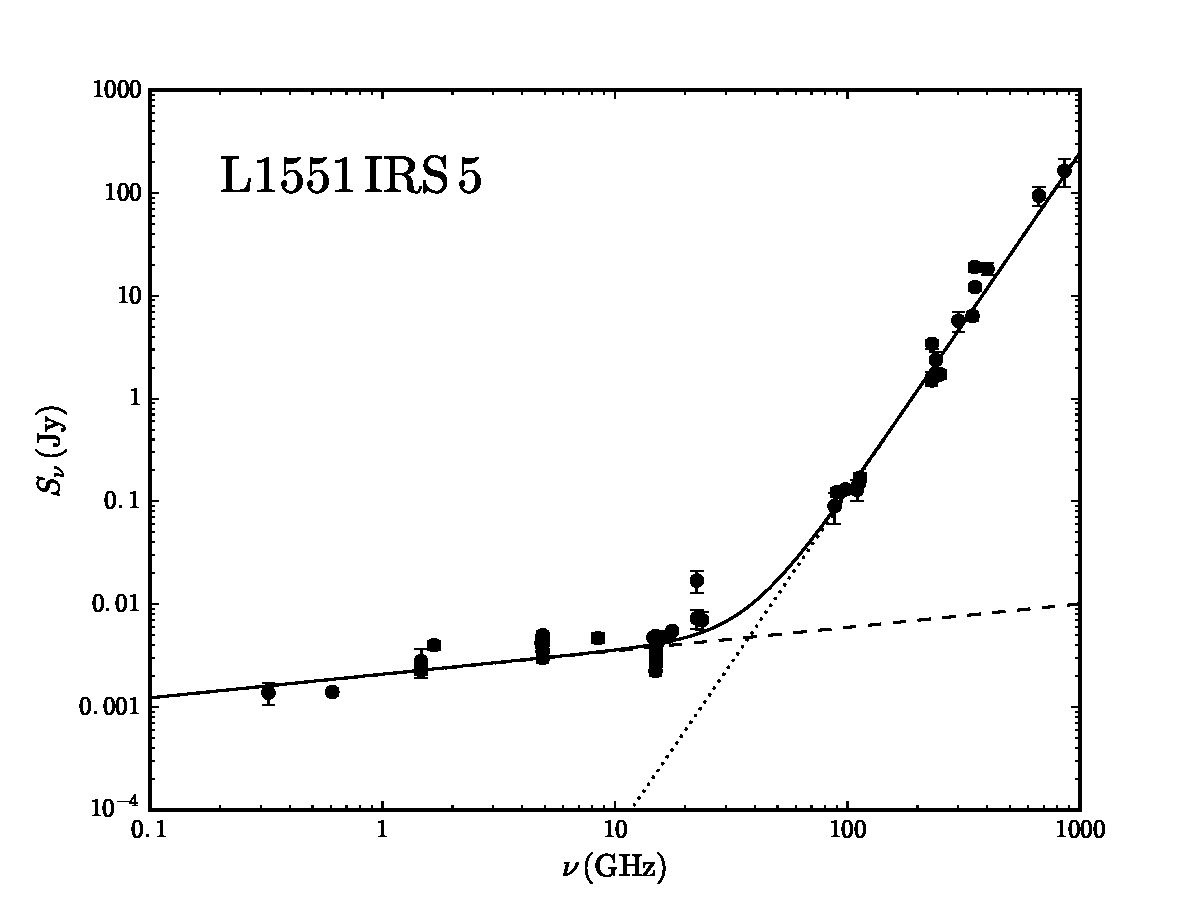
\includegraphics[width=0.65\textwidth]{plots/L1551.pdf}\\
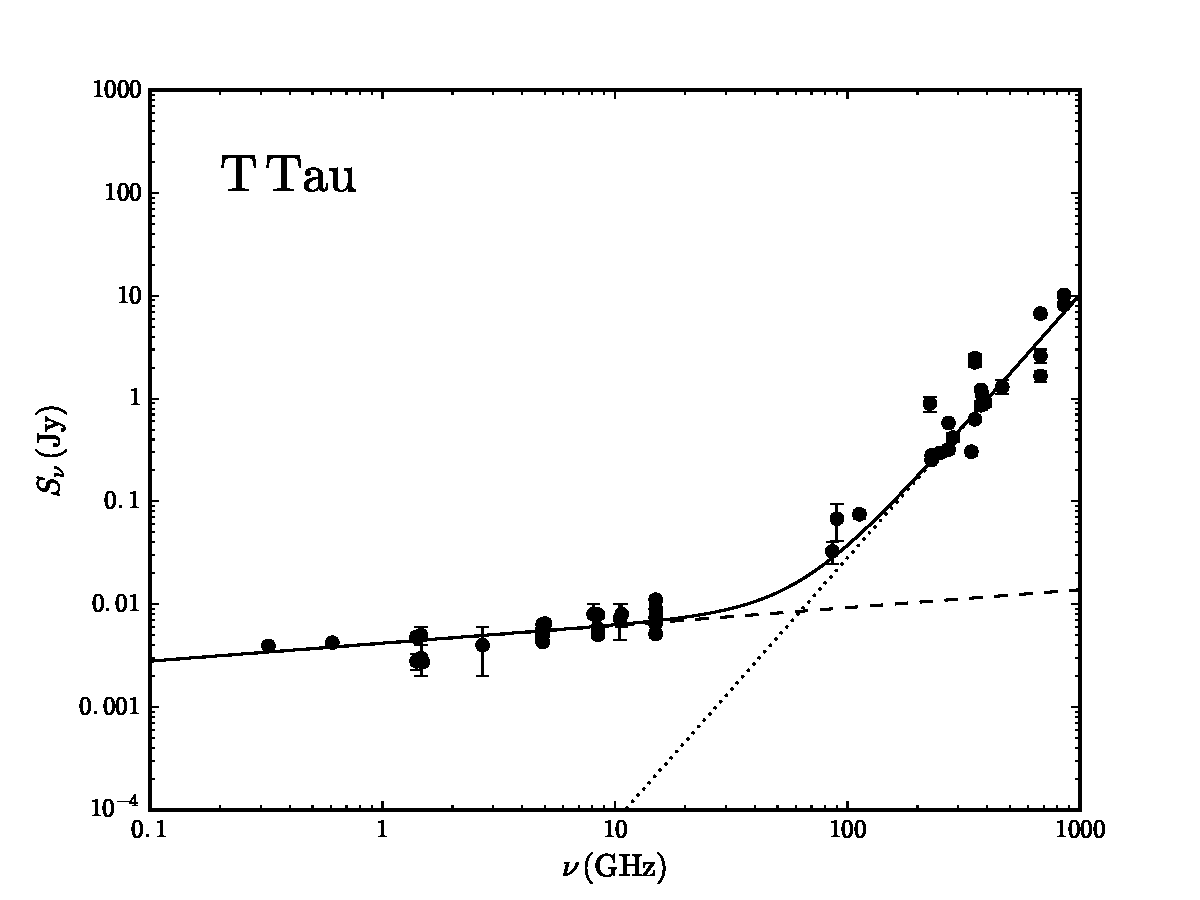
\includegraphics[width=0.65\textwidth]{plots/TTau.pdf}\\
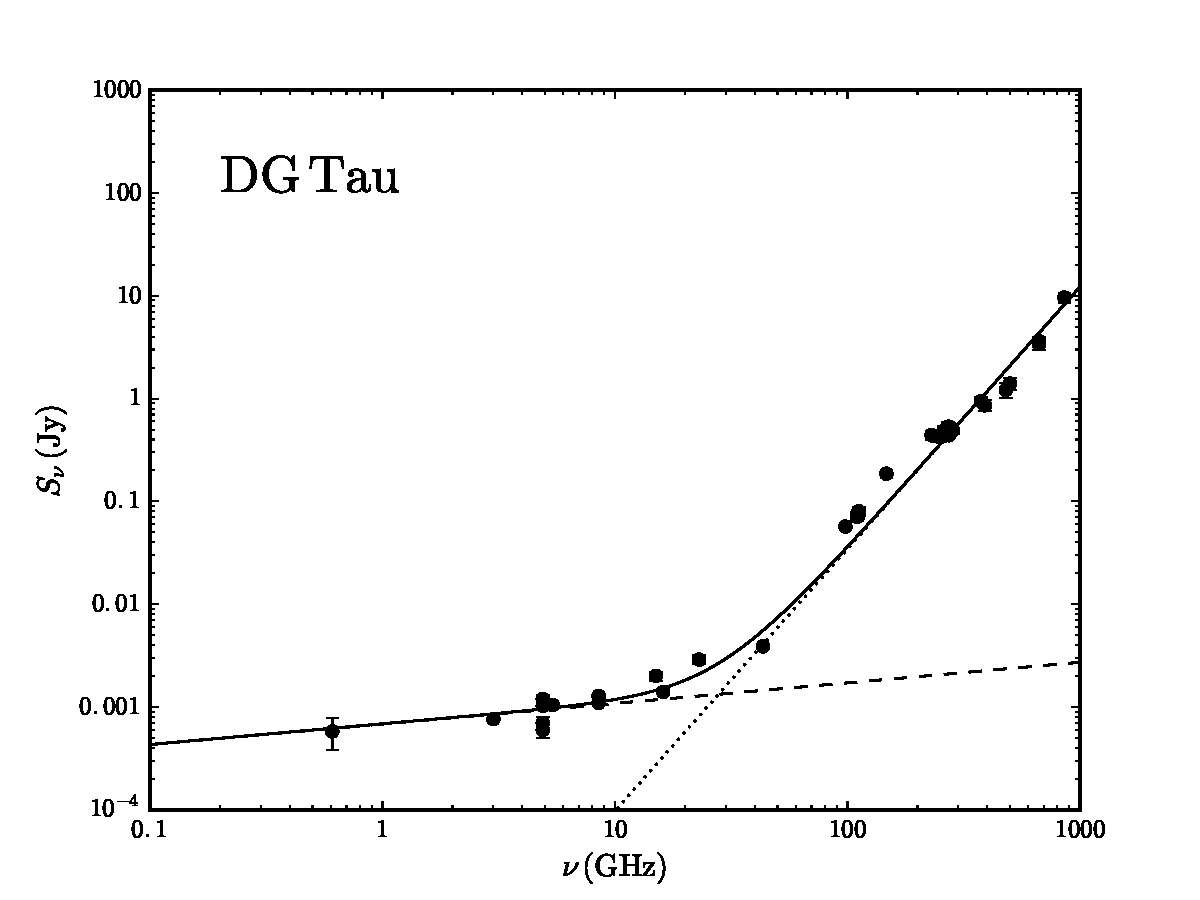
\includegraphics[width=0.65\textwidth]{plots/DGTau.pdf}
\label{default}
\end{center}
\end{figure}



\clearpage



\begin{table}
\caption{T~Tau}
\begin{center}
\begin{tabular}{lllll}
\hline
 $\nu$ & & $S_\nu$ & & Reference\\
 (GHz) & & (mJy) & & \\
\hline
 0.323  &     3.95 & $\pm$ & 0.29  & \citet{2016MNRAS.459.1248A} \\
 0.608  &     4.24 & $\pm$ & 0.23  & \citet{2016MNRAS.459.1248A} \\
 1.4    &     4.80 &    & \dagmark & \citet{1998AJ....115.1693C}\\
 1.4    &     2.80 & $\pm$ & 0.50  & \citet{1986ApJ...303..233S}\\
 1.465  &     5.00 & $\pm$ & 1.00  & \citet{1983RMxAA...8..163R}\\
 1.465  &     3.00 & $\pm$ & 1.00  & \citet{1984ApJ...280L..23S}\\
 1.49   &     2.74 & $\pm$ & 0.11  & \citet{1986AJ.....92.1396C}\\
 2.695  &     4.00 & $\pm$ & 2.00  & \citet{1974ApJ...188L.105S}\\
 4.86   &     4.94 & $\pm$ & 0.34  & \citet{1994AJ....107.1461S}\\
 4.86   &     4.62 & $\pm$ & 0.26  & \citet{1994AJ....107.1461S}\\
 4.86   &     4.53 & $\pm$ & 0.29  & \citet{1994AJ....107.1461S}\\
 4.885  &     5.80 & $\pm$ & 0.60  & \citet{1982ApJ...253..707C}\\
 4.885  &     5.00 & $\pm$ & 0.60  & \citet{1983RMxAA...8..163R}\\
 4.885  &     4.30 & $\pm$ & 0.20  & \citet{1984ApJ...280L..23S}\\
 4.885  &     5.20 & $\pm$ & 0.50  & \citet{1984ApJ...282..699B}\\
 4.885  &     5.70 & $\pm$ & 0.50  & \citet{1986ApJ...303..233S}\\
 4.885  &     6.40 &    & \dagmark & \citet{1987ApJ...320..364E}\\
 5      &     6.50 & $\pm$ & 0.07  & \citet{1982ApJ...253..707C}\\
 8.085  &     8.00 & $\pm$ & 2.00  & \citet{1974ApJ...188L.105S}\\
 8.44   &     5.19 & $\pm$ & 0.30  & \citet{1994AJ....107.1461S}\\
 8.44   &     5.05 & $\pm$ & 0.31  & \citet{1994AJ....107.1461S}\\
 8.44   &     5.79 & $\pm$ & 0.34  & \citet{1994AJ....107.1461S}\\
 8.44   &     7.93 & $\pm$ & 0.51  & \citet{1994AJ....107.1461S}\\
 8.44   &     5.81 & $\pm$ & 0.41  & \citet{1994AJ....107.1461S}\\
 10.5   &     7.30 & $\pm$ & 2.80  & \citet{1979AJ.....84.1709M}\\
 10.69  &     8.00 & $\pm$ & 2.00  & \citet{1976AA....46...11A}\\
 14.94  &     6.50 & $\pm$ & 0.07  & \citet{1986AJ.....92.1396C}\\
 14.949 &     5.14 & $\pm$ & 0.43  & \citet{1994AJ....107.1461S}\\
 14.965 &     9.00 & $\pm$ & 1.00  & \citet{1984ApJ...280L..23S}\\
 14.965 &     7.50 & $\pm$ & 0.70  & \citet{1984ApJ...282..699B}\\
 14.965 &    11.10 & $\pm$ & 1.00  & \citet{1986ApJ...303..233S}\\
 15     &     8.60 & $\pm$ & 2.00  & \citet{1982AA...107..368B}\\
 86     &     32.7 & $\pm$ & 7.8   & \citet{1986AA...164..227A}\\
 90     &     68.0 & $\pm$ & 27.0  & \citet{1977MNRAS.180..297S}\\
 112.6  &     75.0 & $\pm$ & 7.5   & \citet{1989ApJ...344..915W}\\
 226    &     894  & $\pm$ & 153   & \citet{1986AA...164..227A}\\
 230    &     280  & $\pm$ & 9     & \citet{1990AJ.....99..924B}\\
 230    &     253  & $\pm$ & 18    & \citet{1993AA...273..221R}\\
 231    &     280  & $\pm$ & 9     & \citet{2005ApJ...631.1134A}\\
 250    &     296  & $\pm$ & 25    & \citet{1994AA...281..161A}\\
 272    &     320  & $\pm$ & 30    & \citet{1990ApJ...357..606A}\\
 272    &     579  & $\pm$ & 27    & \citet{1989ApJ...340L..69W}\\
 284    &     417  & $\pm$ & 41    & \citet{1991ApJ...381..250B}\\
 341    &     304  &   & \dagmark  & \citet{2012ApJ...751..115H}\\
 353    &    2250  &   & \dagmark  & \citet{2010ApJ...710.1247S}\\
 353    &    2470  &   & \dagmark  & \citet{2008ApJS..175..277D}\\
 353    &      628 & $\pm$ & 17    & \citet{2005ApJ...631.1134A}\\
 375    &     1216 & $\pm$ & 44    & \citet{1989ApJ...340L..69W}\\
 375    &      860 & $\pm$ & 80    & \citet{1994AJ....108..661J}\\
 380    &     1070 & $\pm$ & 110   & \citet{1990ApJ...357..606A}\\
 390    &      910 & $\pm$ & 90    & \citet{1991ApJ...381..250B}\\
 463    &     1300 & $\pm$ & 200   & \citet{1990ApJ...357..606A}\\
 676    &     2600 & $\pm$ & 400   & \citet{1990ApJ...357..606A}\\
 676    &     1655 & $\pm$ & 218   & \citet{2005ApJ...631.1134A}\\
 676    &     6710 & $\pm$ & 610   & \citet{1989ApJ...340L..69W}\\
 854    &    10170 & $\pm$ & 730   & \citet{1989ApJ...340L..69W}\\
 854    &     8149 & $\pm$ & 253   & \citet{2005ApJ...631.1134A}\\
 \end{tabular}
\end{center}
\label{default}
\end{table}%

\clearpage



\begin{table}
\caption{DG~Tau}
\begin{center}
\begin{tabular}{lllll}
\hline
 $\nu$ & & $S_\nu$ & & Reference\\
 (GHz) & & (mJy) & & \\
\hline
 0.608  &  0.58 & $\pm$ & 0.20 & \citet{2016MNRAS.459.1248A}\\
 3.0    &  0.76 & $\pm$ & 0.04 & Ainsworth et~al., in prep.\\
 4.89   &  0.70 & $\pm$ & 0.10 & \citet{1982ApJ...253..707C} \\
 4.89   &  1.20 & $\pm$ & 0.10 & \citet{1984ApJ...282..699B} \\
 4.89   &  1.03 & $\pm$ & 0.07 & \citet{1986AJ.....92.1396C} \\
 4.89   &  0.60 & $\pm$ & 0.10 & \citet{1987ApJ...320..364E} \\
 5.4    &  1.05 & $\pm$ & 0.05 & \citet{2013ApJ...766...53L} \\
 8.5    &  1.27 & $\pm$ & 0.05 & \citet{2012AA...537A.123R} \\
 8.5    &  1.29 & $\pm$ & 0.07 & \citet{2013ApJ...766...53L} \\
 8.5    &  1.10 & $\pm$ & 0.06 & \citet{2013ApJ...766...53L} \\
 15     &  2.01 &  & \dagmark  & \citet{1986AJ.....92.1396C} \\
 16.12  &  1.40 & $\pm$ & 0.07 & \citet{2012MNRAS.420.3334S} \\
 23     &  2.90 &  & \dagmark  & \citet{1982AA...107..368B} \\
 43.3   &  3.90 & $\pm$ & 0.22 & \citet{2013ApJ...766...53L} \\
 98     &  57.0 & $\pm$ & 4.0  & \citet{1991AJ....102.2054O} \\
 110    &  71 &  & \dagmark    & \citet{1989LNP...350..215S} \\
 110    &  72 &  & \dagmark    & \citet{1996ApJ...457..277K} \\
 111    &  75 &  & \dagmark    & \citet{1994ASPC...59..203S} \\
 112    &  80 &  & \dagmark    & \citet{1989ApJ...337L..41W} \\
 147    &  186 & $\pm$ & 17    & \citet{1996ApJ...465L.137K} \\
 230    &  443 &  & \dagmark   & \citet{1990AJ.....99..924B} \\
 230    &  440 &  & \dagmark   & \citet{1990ApJ...357..606A} \\
 250    &  420 & $\pm$ & 42    & \citet{1994AA...281..161A} \\
 260    &  489 &  & \dagmark   & \citet{1991ApJ...381..250B} \\
 270    &  532 &  & \dagmark   & \citet{1989ApJ...340L..69W} \\
 273    &  440 & $\pm$ & 30    & \citet{1990ApJ...357..606A} \\
 273    &  532 & $\pm$ & 48    & \citet{1989ApJ...340L..69W} \\
 284    &  489 & $\pm$ & 33    & \citet{1991ApJ...381..250B} \\
 375    &  940 & $\pm$ & 100   & \citet{1990ApJ...357..606A} \\
 390    &  860 & $\pm$ & 100   & \citet{1991ApJ...381..250B} \\
 480    &  1210 & $\pm$ & 200  & \citet{1991ApJ...381..250B} \\
 500    &  1400 & $\pm$ & 200  & \citet{1990ApJ...357..606A} \\
 666    &  3390 & $\pm$ & 440  & \citet{1989ApJ...340L..69W} \\
 666    &  3600 & $\pm$ & 400  & \citet{1990ApJ...357..606A} \\
 857    &  9600 & $\pm$ & 1100 & \citet{1990ApJ...357..606A} \\
  \end{tabular}
\end{center}
\label{default}
\end{table}%


\clearpage



%%%%%%%%%%%%%%%%%%%% REFERENCES %%%%%%%%%%%%%%%%%%


\bibliographystyle{apj}
\bibliography{Bibliography} % if your bibtex file is called Bibliography.bib


\end{document}  